\documentclass[main]{subfiles}
\begin{document}

%@@@@@@@@@@@@@@@@@@@@@@@@@@@@@@
% Main Topics: Passive Membrane Properties I - 11.10.2018
% Lecturer: Valerio Mante
% author: Vanessa Leite - base document from benelot/eth-intro-to-neuroinformatics-summary

\section{Passive (Cable) Membrane Properties}
\subsection{Basic electronics}
\begin{itemize}[noitemsep,nolistsep]
	\item Ohm's Law: $V = I \cdot R$
	\item Kirchoff's Current Law (KCL): The sum of all currents entering and leaving any node in a circuit is zero.
	\item Kirchoff's Voltage Law (KVL): The sum of all voltages around a closed loop is equal to zero.
\end{itemize}

\subsection{Ion channel replacement circuit}
\begin{itemize}[noitemsep,nolistsep]
	\item Ion channel is equal to resistance.
	\item Ion gradient is equal to battery.
	\item Cell membrane is equal to capacitor.
	\item Conductivity $S=\frac{1}{R}$.
	\item Ion resistance is $R = V/I$.
	\item Ion conductivity is $\gamma = g_L = I/V$.
	\item Outward current for an ion is $I_m=g_L(V-E_L)$.
	\item If the concentration of an ion on one side is raised (with a corresponding molecule of opposite charge) and the membrane is permeable for this ion, then the side which has a higher concentration gets more negative, because the ions go to the other side, leaving behind uncompensated negative charges.
\end{itemize}
\begin{figure}[H]
	\centering
	\scalebox{0.7}{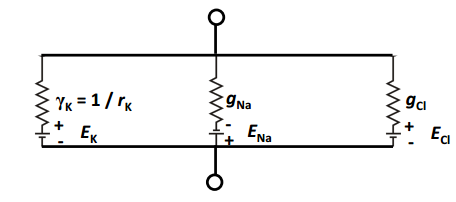
\includegraphics{ion_channel_circuit_01.png}}
\end{figure}
\begin{figure}[H]
	\centering
	\scalebox{0.7}{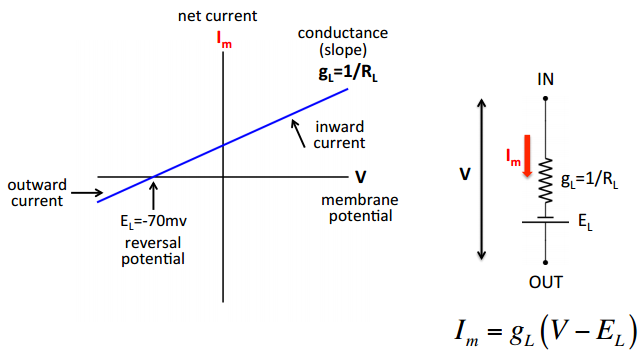
\includegraphics{current_voltage_01.png}}
\end{figure}

\subsection{Single-compartment model}
\subsubsection{Assumptions, configuration}
\begin{itemize}[noitemsep,nolistsep]
	\item Assume isopotential and a sphere of membrane.
	\item $I_e$ is an injected current.
	\item $I_C$ is the capacitive current, discharging the membrane.
	\item There is also a leak current $I_L = g_L(V-E_L)$.
\end{itemize}

\subsubsection{Membrane as electrical circuit}
\begin{itemize}[noitemsep,nolistsep]
	\item $I_e = I_L + I_C$ and $I_L=g_L(V-E_L)$
	\item $C\frac{dV}{dt} = I_C$
	\item $V(t) = V_\infty+(V(0)-V_\infty)e^{-\frac{t}{\tau_m}}$
	\item $V_\infty = E_L + R_LI_e$
	\item Membrane time-constant: $\tau_m = R_LC$
	\item Larger current due to spatial summation.
	\item Less depolarization with small resistance (larger area).
\end{itemize}
\begin{figure}[H]
	\centering
	\begin{subfigure}[b]{0.3\textwidth}
		\centering
		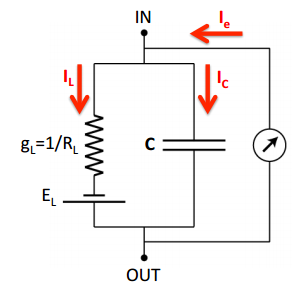
\includegraphics[width=\textwidth]{membrane_circuit_01.png}
	\end{subfigure}%
	~
	\begin{subfigure}[b]{0.5\textwidth}
		\centering
		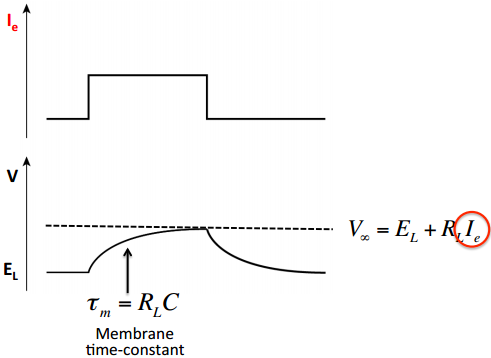
\includegraphics[width=\textwidth]{membrane_circuit_02.png}
	\end{subfigure}
\end{figure}

\subsubsection{Input resistance}
\begin{itemize}[noitemsep,nolistsep]
	\item $A$ is the surface area of the membrane.
	\item $R_L = \frac{r_L}{A}$
\end{itemize}

\subsection{Two ionic currents}
\begin{itemize}[noitemsep,nolistsep]
	\item Equilibrium at $I_L=I_S$
	\item $V_\infty = \frac{g_LE_L+g_SE_S}{g_L+g_S}$
	\item $\tau_m = \frac{C}{g_L+g_S}$
\end{itemize}
\begin{figure}[H]
	\centering
	\begin{subfigure}[b]{0.4\textwidth}
		\centering
		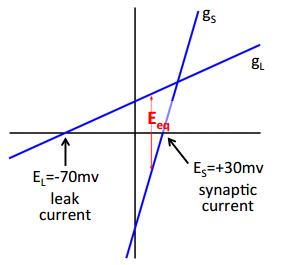
\includegraphics[width=\textwidth]{current_voltage_02.png}
	\end{subfigure}%
	~
	\begin{subfigure}[b]{0.4\textwidth}
		\centering
		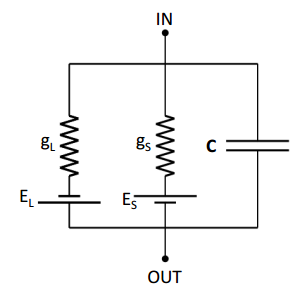
\includegraphics[width=\textwidth]{membrane_circuit_03.png}
	\end{subfigure}
\end{figure}

\subsection{The cable equation}
\[c_m\frac{\partial V}{\partial t} = \frac{1}{2ar_L}\frac{\partial}{\partial x}(a^2\frac{\partial V}{\partial x})-i_m+i_e\]
\begin{figure}[H]
	\centering
	\scalebox{0.7}{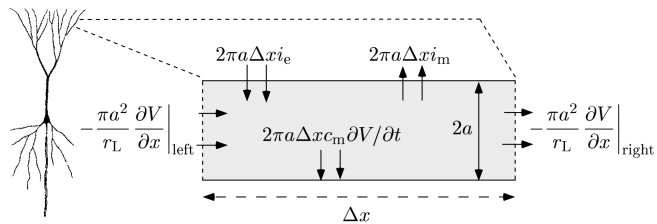
\includegraphics{cable_equation_01.png}}
\end{figure}
\subsubsection{Infinite cable}
\begin{figure}[H]
	\centering
	\scalebox{0.7}{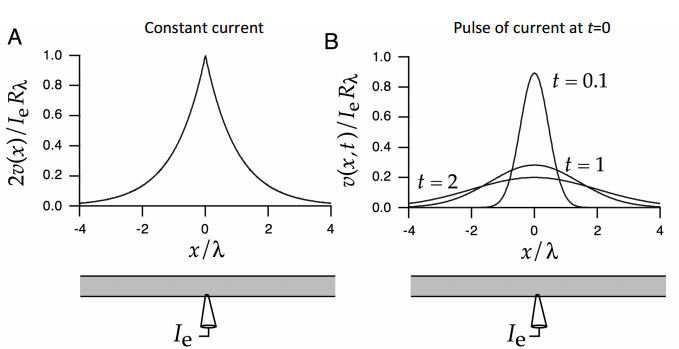
\includegraphics{cable_equation_02.png}}
\end{figure}
\begin{itemize}[noitemsep,nolistsep]
	\item $v(x) = \frac{I_eR_\lambda}{2}\exp(-\frac{|x|}{\lambda})$
	\item $R_\lambda=\frac{r_m}{2\pi a\lambda} = \frac{r_L\lambda}{\pi a^2}$
	\item $\lambda = \sqrt{\frac{ar_m}{2r_L}}$ sets the scale for the spatial variation in the membrane potential.
	\item $\lambda$ is the electronic length, or how far the signal travels.
	\item $\tau_m = r_mc_m$ sets the scale for the temporal variation in the membrane potential.
	\item $v(x,t) = \frac{I_eR_\lambda}{\sqrt{4\pi\lambda^2t/\tau_m}}\exp(-\frac{\tau_mx^2}{4\lambda^2t})\exp(-\frac{t}{\tau_m})$
	\item $a$ is the radius of the axon, about $2\,\mu m$
	\item $r_m$ is the specific membrane resistance, about $1\,M\Omega\cdot mm^2$
	\item $v = V - V_{rest}$
	\item $r_L$ is the longitudinal resistance, about $1\,k\Omega\cdot mm$
	\item $I_e$ is the injected current.
	\item It follows, that increasing $R_m$ also increases $\lambda$. With better isolation, signals travel further.
	\item Increasing the diameter also increases $\lambda$.
\end{itemize}

\subsection{Level of approximation}
\begin{itemize}[noitemsep,nolistsep]
	\item A neuron can be represented by a variable number of discrete compartments.
	\item Compartments represent a region, each with a single membrane potential.
	\item The connections between compartments have resistive couplings.
\end{itemize}

\subsection{Hodgkin-Huxley Equations}
\begin{itemize}[noitemsep,nolistsep]
	\item Model that describes how action potentials in neurons are initiated and propagated.
	\item $n$ and $m$ are probabilities for a gate to be open.
	\item $h$ is the probability that an open channel is not blocked.
	\item The gating variables have a voltage dependence.
	\item $\bar{g}$ values are the maximum conductance possible.
	\item There is no inactivation for potassium, only for sodium.
	\item The membrane does not get locked at positive values.
	\item $\bar{g}_L$ stands for some generic leak.
	\item The functions $n_\infty(V)$, $m_\infty(V)$ and $h_\infty(V)$ determine whether gates serve to activate channels (with depolarization) or inactivate the channel (close with depolarization). $\tau_m$, $\tau_h$ and $\tau_n$ are time constants.
\end{itemize}
\[C\frac{dV}{dt}+\bar{g}_Kn^4(V-V_K)+\bar{g}_{Na}m^3h(V-V_{Na})+\bar{g}_L(V-V_L)+I_{inj}=0\]

\begin{figure}[H]
	\centering
	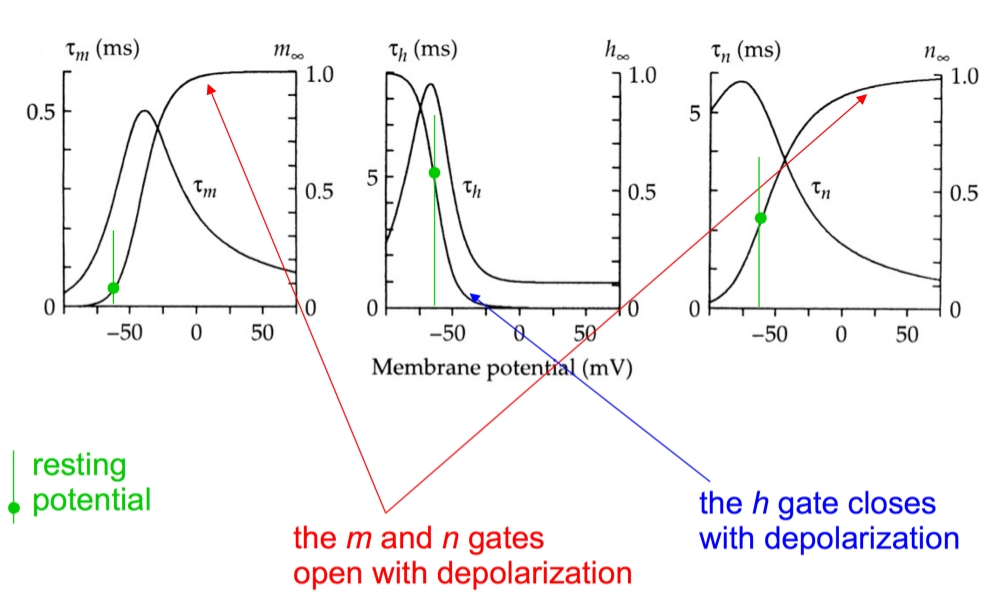
\includegraphics[scale=0.5]{5_8.jpg}
\end{figure} 
\begin{figure}[H]
	\centering
	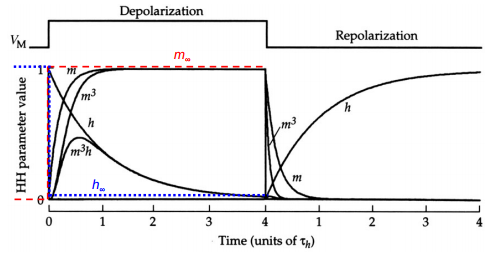
\includegraphics[scale=1.0]{depolarization_01.png}
\end{figure} 



\end{document}
